% =============================================================================
% Algebra 2 — Lesson 4-4: Adding and Subtracting Rational Expressions
% Converted from the Savvas enVision Algebra 2 lesson packet.
% Compile with pdflatex (requires the train image in ./media/image3.png).
% =============================================================================
\documentclass[11pt]{article}

% --- Page setup --------------------------------------------------------------
\usepackage[letterpaper,margin=0.9in,top=1.0in,headheight=14pt]{geometry}
\usepackage{fancyhdr}
\pagestyle{fancy}
\fancyhf{}
\fancyhead[L]{\small Algebra 2 -- Block \underline{\hspace{1.0cm}}\ \
Date \underline{\hspace{2.0cm}}\ \
Name \underline{\hspace{5.5cm}}}
\fancyfoot[R]{\small\thepage}
\renewcommand{\headrulewidth}{0pt}

% --- Math & symbols ----------------------------------------------------------
\usepackage{amsmath, amssymb}

% --- Color + highlighting ----------------------------------------------------
\usepackage{xcolor}
\usepackage{tcolorbox}
\definecolor{examplebg}{RGB}{178,235,242}
\definecolor{accentblue}{RGB}{0,150,210}
\definecolor{accentred}{RGB}{195,55,70}

% --- Graphics ----------------------------------------------------------------
\usepackage{graphicx}
\graphicspath{{media/}}

% --- Tables ------------------------------------------------------------------
\usepackage{array}
\usepackage{tabularx}

% --- Lists -------------------------------------------------------------------
\usepackage{enumitem}
\setlist[itemize]{itemsep=2pt, topsep=3pt, leftmargin=*}
\setlist[enumerate]{itemsep=2pt, topsep=3pt, leftmargin=*}

% --- Custom commands ---------------------------------------------------------
\newcommand{\blank}[1][1.2cm]{\underline{\hspace{#1}}}

% Highlighted example header (cyan banner)
\newcommand{\examplehead}[1]{%
  \bigskip\noindent%
  \begin{tcolorbox}[colback=examplebg,colframe=examplebg,boxrule=0pt,
                    left=5pt,right=5pt,top=3pt,bottom=3pt,arc=1pt]%
    \large\bfseries #1%
  \end{tcolorbox}\smallskip}

\newcommand{\sidequestion}[1]{%
  \smallskip\noindent\textit{\small #1}\par}

\setlength{\parindent}{0pt}
\setlength{\parskip}{4pt}

\begin{document}

% =============================================================================
% TITLE + OBJECTIVES
% =============================================================================
\begin{center}
  {\LARGE\bfseries Lesson 4-4: Adding and Subtracting Rational Expressions}
\end{center}

\renewcommand{\arraystretch}{1.3}
\begin{tabularx}{\textwidth}{|>{\bfseries\raggedright\arraybackslash}p{3.4cm}|X|}
\hline
Math Objective & Understand that rational expressions form a system analogous to
the system of rational numbers and use that understanding to add and subtract
rational expressions. \\ \hline
Language Objective & Students will build rational expressions for a $d=rt$ word
problem using a graphic organizer. \\ \hline
Essential Question & I can find the sum or difference of rational expressions. \\ \hline
\end{tabularx}
\renewcommand{\arraystretch}{1.0}

% =============================================================================
% CRITIQUE & EXPLAIN
% =============================================================================
\bigskip
{\large\bfseries\color{accentblue}CRITIQUE \& EXPLAIN}

Teo and Evander find the following exercise in their homework:
\[ \tfrac{1}{2} \;+\; \tfrac{1}{3} \;+\; \tfrac{1}{9} \]

\textbf{A.}\quad Teo claims that a common denominator of the sum is
$2+3+9 = 14$. Evander claims that it is $2\cdot 3 \cdot 9 = 54$. Is either
student correct? Explain why or why not.
\vspace{2.2cm}

\textbf{B.}\quad Find the sum, explaining the method you use.
\vspace{2.2cm}

\textbf{C.}\ \textcolor{accentred}{\textbf{Construct Arguments}}\ \
Timothy states that the quickest way to find the sum of any two fractions with
unlike denominators is to multiply their denominators to find a common
denominator, and then rewrite each fraction with that denominator. Do you agree?
\vspace{2.2cm}

% --- Habits of Mind ---
\noindent\rule{\textwidth}{0.3pt}

\textcolor{accentred}{\textbf{HABITS OF MIND}}\quad
\textbf{Look for Relationships}\ \
For two fractions with denominators $10$ and $x$, when is $10x$ the least
common multiple? When is $10x$ \textit{not} the least common multiple?
\vspace{2cm}

\newpage

\sidequestion{What do you notice about the expression in the exercise?}
\vspace{1.2cm}

\sidequestion{How can there be more than one answer to the problem?}
\vspace{1.2cm}

% =============================================================================
% EXAMPLE 1 — Like Denominators
% =============================================================================
\examplehead{EXAMPLE 1 --- Add or Subtract Rational Expressions with Like Denominators}

When rational expressions have the same denominator, we combine the numerators
and keep the denominator the same. This procedure is just like numerical
fractions.
\[ \frac{x+5}{x+4} + \frac{3}{x+4} \]

\textbf{Since both fractions have the denominator $x+4$, we add the numerators:}
\[ \frac{x+5+3}{x+4} \;=\; \frac{x+8}{x+4} \]

\sidequestion{Explain why it does not make sense to add the denominators?}
\vspace{1.6cm}

\textbf{Domain:}\quad The denominator $x+4$ cannot be zero, so
\[ x \neq -4 \]

% --- TRY IT 1 ---
\medskip
\textbf{TRY IT 1}\quad Add or subtract the rational expressions. Then state the domain.

\renewcommand{\arraystretch}{1.3}
\begin{tabularx}{\textwidth}{|>{\raggedright\arraybackslash}X|>{\raggedright\arraybackslash}X|}
\hline
\begin{minipage}[t][5.2cm][t]{\linewidth}
\centering\vspace{0.15cm}
$\displaystyle \frac{4}{3x+1} \;+\; \frac{x+9}{3x+1}$

\vspace{2.2cm}
\raggedright\textbf{Simplified form:}

\vspace{0.9cm}
\textbf{Domain:}\ \ $x \neq \blank[1.2cm]$
\end{minipage}
&
\begin{minipage}[t][5.2cm][t]{\linewidth}
\centering\vspace{0.15cm}
$\displaystyle \frac{2x-3}{x-7} \;-\; \frac{5}{x-7}$

\vspace{2.2cm}
\raggedright\textbf{Simplified form:}

\vspace{0.9cm}
\textbf{Domain:}\ \ $x \neq \blank[1.2cm]$
\end{minipage}
\\ \hline
\end{tabularx}
\renewcommand{\arraystretch}{1.0}

% =============================================================================
% EXAMPLE 2 — Find the LCD
% =============================================================================
\examplehead{EXAMPLE 2 --- Find the LCD of Rational Expressions}

To add or subtract rational expressions, we first need a
\textbf{common denominator}. When denominators are factored, the \textbf{LCD}
is the product of all unique factors.

Find the \textbf{LCD} of:
\[ \frac{7}{x+4} \qquad \text{and} \qquad \frac{3}{(x+4)(x-6)} \]

\textbf{Step 1 --- Identify factors}
\begin{itemize}
  \item First denominator:\ \ $x+4$
  \item Second denominator:\ \ $(x+4)(x-6)$
\end{itemize}

\textbf{Step 2 --- Combine all unique factors}
\[ \text{LCD:}\quad (x+4)(x-6) \]

\sidequestion{Why didn't we include $x+4$ twice?}
\vspace{1.4cm}

% --- TRY IT 2 ---
\textbf{TRY IT 2}\quad Find the LCD of the following rational expressions:

\renewcommand{\arraystretch}{1.3}
\begin{tabularx}{\textwidth}{|>{\raggedright\arraybackslash}X|>{\raggedright\arraybackslash}X|}
\hline
\begin{minipage}[t][4.5cm][t]{\linewidth}
\centering\vspace{0.15cm}
$\displaystyle \frac{5}{x+2} \quad \text{and} \quad \frac{9}{(x+2)(x-5)}$

\vspace{2.5cm}
\raggedright\textbf{LCD:}
\end{minipage}
&
\begin{minipage}[t][4.5cm][t]{\linewidth}
\centering\vspace{0.15cm}
$\displaystyle \frac{3}{x-1} \quad \text{and} \quad \frac{5}{x^{2}-1}$

\textit{Difference of squares!}

\vspace{1.9cm}
\raggedright\textbf{LCD:}
\end{minipage}
\\ \hline
\end{tabularx}
\renewcommand{\arraystretch}{1.0}

% =============================================================================
% EXAMPLE 3 — Unlike Denominators
% =============================================================================
\examplehead{EXAMPLE 3 --- Add or Subtract Rational Expressions with Unlike Denominators}

When rational expressions have \textbf{different denominators}, the process is
the same whether you are adding or subtracting:
\begin{enumerate}
  \item \textbf{Find the LCD}
  \item \textbf{Rewrite each fraction using the LCD}
  \item \textbf{Combine the numerators} (add or subtract)
  \item \textbf{State the domain}
\end{enumerate}

% --- Example A: Addition ---
\smallskip
\underline{\textbf{Example A --- Addition}}
\[ \frac{5}{x+3} \;+\; \frac{x-2}{(x+3)(x-1)} \]

\textbf{Step 1: LCD}
\[ (x+3)(x-1) \]

\textbf{Step 2: Rewrite}
\[ \frac{5}{x+3} \cdot \frac{x-1}{x-1} \;=\; \frac{5(x-1)}{(x+3)(x-1)} \]

\sidequestion{Why are we allowed to change fractions before adding them?}
\vspace{1.2cm}

Second fraction already has the LCD.

\textbf{Step 3: Add}
\[ \frac{5(x-1) + (x-2)}{(x+3)(x-1)} \]

Simplify numerator:
\[ 5x - 5 + x - 2 \;=\; 6x - 7 \]

\textbf{Final Answer}
\[ \frac{6x-7}{(x+3)(x-1)} \]

\textbf{Domain}
\[ x \neq -3, \qquad x \neq 1 \]

% --- Example B: Subtraction ---
\bigskip
\underline{\textbf{Example B --- Subtraction}}
\[ \frac{x+7}{x-3} \;-\; \frac{4}{x+2} \]

\textbf{Step 1: LCD}
\[ (x-3)(x+2) \]

\textbf{Step 2: Rewrite}
\[ \frac{x+7}{x-3} \cdot \frac{x+2}{x+2} \;=\; \frac{(x+7)(x+2)}{(x-3)(x+2)} \]
\[ \frac{4}{x+2} \cdot \frac{x-3}{x-3} \;=\; \frac{4(x-3)}{(x-3)(x+2)} \]

\textbf{Step 3: Subtract}
\[ \frac{(x+7)(x+2) \;-\; 4(x-3)}{(x-3)(x+2)} \]

Expand:
\[ (x+7)(x+2) \;=\; x^{2} + 9x + 14 \]
\[ 4(x-3) \;=\; 4x - 12 \]

Subtract:
\[ x^{2} + 9x + 14 \;-\; (4x - 12) \]

\textit{Be careful with the subtraction:}
\[ x^{2} + 9x + 14 - 4x + 12 \;=\; x^{2} + 5x + 26 \]

\textbf{Final Answer}
\[ \frac{x^{2} + 5x + 26}{(x-3)(x+2)} \]

\textbf{Domain}
\[ x \neq 3, \qquad x \neq -2 \]

\smallskip
\sidequestion{What extra step(s) do we need here that we don't do with regular fractions?}
\vspace{1.4cm}

\sidequestion{How is the distributive property used when subtracting rational expressions?}
\vspace{1.4cm}

% --- TRY IT 3 ---
\textbf{TRY IT 3}

\renewcommand{\arraystretch}{1.3}
\begin{tabularx}{\textwidth}{|>{\raggedright\arraybackslash}X|>{\raggedright\arraybackslash}X|}
\hline
\begin{minipage}[t][7.5cm][t]{\linewidth}
\textbf{Add these expressions}
\[ \frac{4}{x-5} + \frac{x+3}{(x-5)(x+1)} \]
\vspace{3.0cm}

\textbf{Simplified form:}

\vspace{0.9cm}
\textbf{Domain:}\ \ $x \neq \blank,\ \ x \neq \blank$
\end{minipage}
&
\begin{minipage}[t][7.5cm][t]{\linewidth}
\textbf{Subtract these expressions}
\[ \frac{x-8}{x+4} \;-\; \frac{6}{x+6} \]
\vspace{3.0cm}

\textbf{Simplified form:}

\vspace{0.9cm}
\textbf{Domain:}\ \ $x \neq \blank,\ \ x \neq \blank$
\end{minipage}
\\ \hline
\end{tabularx}
\renewcommand{\arraystretch}{1.0}

% =============================================================================
% EXAMPLE 5 — Word Problem
% =============================================================================
\examplehead{EXAMPLE 5 --- Use Rational Expressions to Solve Problems}

Jorge drives his car to the mechanic, then he takes the commuter rail train
back to his neighborhood. The average speed for the $10$-mile trip is
$15$ miles per hour faster on the train. Find an expression for Jorge's total
travel time. If he drove $30$ mph, how long did this take?

\begin{center}
  % Comment out this line if compiling without the image file.
  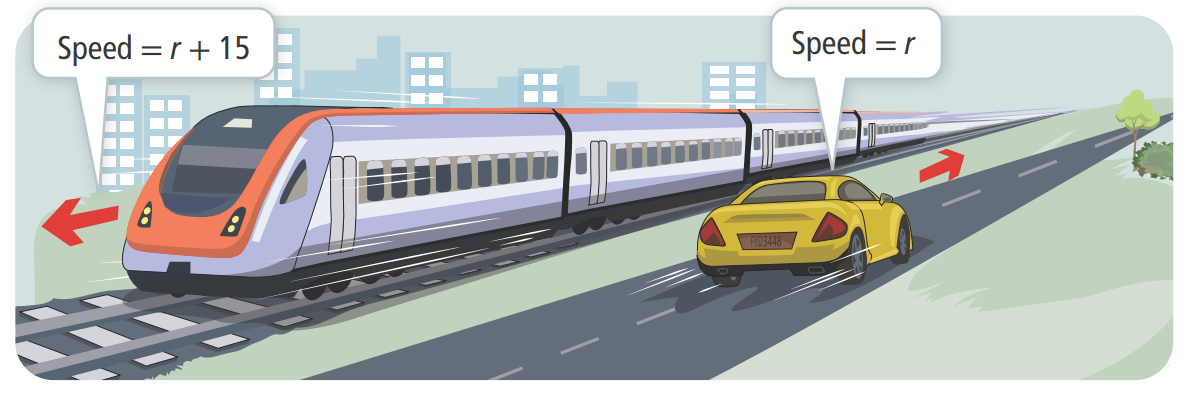
\includegraphics[width=0.92\textwidth]{image3.png}
\end{center}

\medskip
% d = rt organizer
\renewcommand{\arraystretch}{2.6}
\begin{tabularx}{\textwidth}{|>{\centering\arraybackslash}p{2.5cm}|>{\centering\arraybackslash}X|>{\centering\arraybackslash}X|>{\centering\arraybackslash}X|}
\hline
 & \textbf{Distance} & \textbf{Rate} & \textbf{Time} \\ \hline
\textbf{Car}   &  &  &  \\ \hline
\textbf{Train} &  &  &  \\ \hline
\end{tabularx}
\renewcommand{\arraystretch}{1.0}

\medskip
\sidequestion{How do you know you need to add these expressions to solve the problem?}
\vspace{1.2cm}

\sidequestion{What does each fraction represent in the context?}
\vspace{1.2cm}

\sidequestion{How is a table a useful tool in solving this problem?}
\vspace{1.2cm}

% --- TRY IT 5 ---
\textbf{TRY IT --- 5}\quad Jorge drives to visit his friends. His $20$-mile
trip to their house is congested with traffic, but it has cleared by the time
he travels home. He can travel $5$ miles per hour faster. Write an expression
that represents Jorge's total travel time.
\vspace{3.5cm}

% =============================================================================
% SELECT EXERCISES
% =============================================================================
\newpage
\begin{center}
  {\Large\bfseries Select Exercises}
\end{center}

\renewcommand{\arraystretch}{1.3}
\begin{tabularx}{\textwidth}{|>{\raggedright\arraybackslash}p{7.2cm}|X|}
\hline
% --- 3. Error Analysis ---
\textbf{3.}\ \textcolor{accentred}{\textbf{Error Analysis}}\ \
A student added the rational expressions as follows:
\[ \frac{5x}{x+7} + \frac{7}{x} \;=\; \frac{5x}{x+7} + \frac{7(7)}{x+7} \;=\; \frac{5x+49}{x+7} \]
Describe and correct the error the student made.
\hfill\textbf{DOK2}
&
\vspace{4.2cm}
\\ \hline
% --- 12. Generalize ---
\textbf{12.}\ \textcolor{accentred}{\textbf{Generalize}}\ \
Explain how addition and subtraction of rational expressions is similar to and
different from addition and subtraction of rational numbers.
\hfill\textbf{DOK2}
&
\vspace{3.2cm}
\\ \hline
% --- 35. SAT/ACT ---
\textbf{35.}\ \textcolor{accentred}{\textbf{SAT/ACT}}\ \
What is the difference between $\dfrac{x}{9}$ and $\dfrac{x-y}{6}$?

\smallskip
\begin{tabular}{@{}ll@{\hspace{0.7cm}}ll@{}}
\textcircled{\scriptsize A} & $\dfrac{5x-y}{18}$ &
\textcircled{\scriptsize B} & $\dfrac{5x+y}{18}$  \\[10pt]
\textcircled{\scriptsize C} & $\dfrac{-x+3y}{18}$ &
\textcircled{\scriptsize D} & $\dfrac{-x-3y}{18}$
\end{tabular}
\hfill\textbf{DOK1}
&
\vspace{3.5cm}
\\ \hline
% --- 26. Bike trail ---
\textbf{26.}\quad On Saturday morning, Ahmed decided to take a bike ride from
one end of the $15$-mile bike trail to the other end of the bike trail and
back. His average speed the first half of the ride was $2$ mph faster than his
speed on the second half. Find an expression for Ahmed's total travel time.
If his average speed for the first half of the ride was $12$ mph, how long was
Ahmed's bike ride?\ \ \textsc{\small See Example 5}
\hfill\textbf{DOK2}
&
\vspace{4.8cm}
\\ \hline
% --- 31. Use Structure ---
\textbf{31.}\ \textcolor{accentred}{\textbf{Use Structure}}\ \
Aisha paddles a kayak $5$ miles downstream at a rate $3$ mph faster than the
river's current. She then travels $4$ miles back upstream at a rate $1$ mph
slower than the river's current.\ \textit{Hint: Let $x$ represent the rate of
the river current.}

\textbf{a.}\ Write and simplify an expression to represent the total time it
takes Aisha to paddle the kayak $5$ miles downstream and $4$ miles upstream.

\textbf{b.}\ If the rate of the river current, $x$, is $2$ mph, how long was
Aisha's entire kayak trip?
\hfill\textbf{DOK3}
&
\vspace{5.5cm}
\\ \hline
\end{tabularx}
\renewcommand{\arraystretch}{1.0}

\end{document}
